\documentclass[11pt, letterpaper, twoside]{article}
\usepackage[utf8]{inputenc}
\usepackage[T1]{fontenc}
\usepackage{fancyhdr}
\usepackage[margin=1in, include foot]{geometry}
\usepackage{ragged2e}
\usepackage[]{hyperref}
\usepackage{apacite}
\usepackage{setspace}
\usepackage{caption}
\usepackage{subcaption}
\usepackage{etoolbox}
\usepackage{graphicx}
\usepackage{amsmath, amssymb}
\usepackage{cleveref}
\usepackage{wrapfig}
\usepackage{afterpage}
\usepackage{floatrow}
\usepackage{tikz}
\usepackage{booktabs}

\setlength{\parindent}{0pt}
\title{\singlespacing\textbf{November 1, 2021: Status of \textit{The Economist} Leader-Sentiment-Earnings Project}}

\author{Joshua Y. Levy \thanks{Joshua Y. Levy  (joshua.levy@chicagobooth.edu), Stigler Center, Booth School of Business, University of Chicago}}
\date{\today}

\doublespacing
\begin{document}
\begin{titlepage}
    \maketitle
    \thispagestyle{empty}
\end{titlepage}


\newpage
\pagenumbering{arabic}

\section{Introduction to this Document}
Since the beginning of August, I have been working on a project that tries to identify the role business-facing publications in the ``revolving door'' phenomenon between government and the private sector. In an effort to summarize the results of this project to date, I have produced this document which does the following. First it outlines the motivating argument underlying the project, and identifies how the project has evolved over the past three months. Subsequently, it identifies some key results that have driven the methodological evolution of the project and the challenges associated with those various methods. Finally, in this document, I make the case that this project  --- as it is currently conceived --- likely cannot completed accurately with any degree of assurance that the underlying results would be 1) accurate; 2) replicable; or 3) externally valid.

\section{Hypothesis and Argument}
Modern democracies exhibit strong ``revolving door'' phenomena whereby government officials often leave their posts for more lucrative opportunities in the private sector. Taken to its natural extension this phenomena raises the question: what do world leaders do after they leave office?\\

Anecdotally, there is plenty of evidence of former presidents and prime ministers establishing NGOs, joining boards of private corporations, becoming consultants, writing books, and racking up large fees on the speaking circuit. A subsequent question arises: why can some leaders make more than others?\\

In the revolving door setting, we suppose that business-facing publications (which cater to the business elite) serve as an important intermediary. Publications like \textit{The Economist}, \textit{Financial Times}, and \textit{Wall Street Journal} provide informative signals to business leaders as to the pro-business \textit{bona fides} of world leaders. In turn, businesses are willing to pay more in consulting fees and board compensation to former world leaders they perceive as being more business-friendly or more amenable to the objectives of the corporation.\\

We consider the former leaders of only substantively democratic nations for two reasons. First, substantive democracies tend to be more transparent --- suggesting that the press has a bigger role in those nations relative to autocratic ones. Indeed, in many settings, freedom of the press is considered one of the necessary constituent parts of substantive democracy. Additionally, when considering former leaders of autocratic or authoritarian nations, businesses may be inclined to access or retain former leaders not because of the supposed competence of the leader in question as conveyed by the press, but because of the perception that doing so is either necessary or advantageous for practicing some kind of (illicit) corruption. For the question at hand, it would be difficult to isolate the effect of this ``illicit corruption'' channel from the one of interest --- the role of business-facing news publications.\\

\textsc{\textbf{HYPOTHESIS: }} We suppose that the sentiment expressed by \textit{The Economist} is a predictor of the post-term (out-of-office) earnings of former democratic world leaders. That is, the more positively \textit{The Economist} writes about a leader, the more that leader is able to command (or the more businesses are willing to pay) in compensation for out-of-office services.

\section{Sentiment Analysis Tools}
After data collection, to date, work on this project has primarily focussed on conducting sentiment analysis on \textit{The Economist}. This work can be divided into three periods generally defined by the sentiment analysis tools used: SentimentR, VADER, and BART.

\subsection{SentimentR}
    The first tool that I used to evaluate sentiment is called SentimentR. SentimentR relies on a valence-shifter-aware dictionary-based approach to sentiment analysis. This is one degree more sophisticated than a naive dictionary approach which takes a (weighted) average of pre-assigned ``polarity scores'' for the words in a sentence.\footnote{These dictionaries often include common idioms that have scores assigned at the idiom-level rather than the word-level.} Valence shifters are important because they can have significant effects on the expressed sentiment. For instance, the word \verb|not| is a ``negator'' that ``negates'' the sign on the sentiment score assigned to a sentence like: \verb|I do not like ice cream.| Other classes of valence shifters include amplifiers, de-amplifiers, and adversative conjunctions.\\

    Importantly, SentimentR scores text at the sentence-level. Even an article that exclusively profiles a single leader is unlikely to identify that leader in every sentence. Instead, for the purposes of style, copy writers might use:
    \begin{itemize}
        \item Pronouns and titles: For example \verb|She| instead of \verb|Angela Merkel|;
        \item Metonymy: For example \verb|the Blue House| instead of \verb|Moon Jae-In|;\footnote{Metonymy is the linguistic device of invoking one thing to refer to something related.} or
        \item Synecdoche: For example \verb|Washington| instead of \verb|the administration of Donald Trump.|\footnote{Synecdoche is subset of metonymy, often using a part a part of a thing as a stand-in for the broader concept.}
    \end{itemize}
    Important, sentiment-bearing information may be included in such sentences. In order to address this problem I use a Natural Language Processing (NLP) technique called coreference resolution (more details below). This process is intended to maximize the number of sentences that could be tagged as a ``leader-sentence'' (i.e. a sentence that implicitly or explicitly mentions a leader of interest.).\\

    The process of segregating leader-sentences from ``ambient-sentences'' is important for extracting sentiment expressed by \textit{The Economist} about the leader in particular as opposed to the sentiment expressed by \textit{The Economist} about the article in general. This becomes particularly acute in the cases of an ``event- '' or ``disaster- '' bias (more details in Section 5). In addition to computing sentence-level sentiment, I aggregate to the ``entity-level'' to have two numbers statistic that represent the sentiment expressed by an article about the leader of interest, and the ``ambient'' sentiment expressed by the article. SentimentR returns scores ranging from $-1$, most negative to $1$, most positive.

    \subsubsection{AllenNLP Coreference Resolution}
    Coreference resolution is an NLP technique for identifying repeated expressions or references of a single entity in a large (i.e. multi-sentence) body of text. This is often an important step in higher-level NLP tasks such as text summarization, question answer, and other reading comprehension problems.\\

    In our case, we us it narrowly for the purposes of cluster and span replacement. The particular model that I use, SpanBERT, identifies ``clusters,'' or entities, within a body of text and associates ``spans,'' or text-segments, with those clusters. If an identified cluster matches the leader of interest, I can replace all of the identified spans with the leader's name to increase the number of leader-sentences available for sentiment analysis.\\
    
\subsection{VADER}
    Valence Aware Dictionary and sEntiment Reasoner (VADER) is similar in approach to SentimentR. This was additionally used as a sort of robustness check to ensure that sentiment analysis results produced by SentimentR were consistent.\\

    Because VADER also evaluates text at the sentence-level, the same coreference resolution process as described above is used prior to evaluation. Following sentence-level evaluation, the same entity-level aggregation process is used to determine the average leader sentiment and average ambient sentiment. Additionally, VADER also returns scores ranging from $-1$ to $1$.
    
\subsection{BART}
    Finally, I used a pre-trained BART model for sentiment analysis. Unlike SentimentR and VADER, BART represents a machine-learning approach. It is of critical importance to note that BART was not trained for sentiment analysis, but instead trained for text-classification.\\

    That is, in being trained on a hand-labelled corpus of text, BART develops a (very) high dimensional representation of the word embeddings that constitutes those labels. The high-dimensionality of this space permits for implicit ``topics'' or ``clusters'' to develop even for concepts that were not in the labelled training set. In prediction, BART attempts to identify the cluster that is most closely associated with the text of interest.\\

    For our purposes, I attempt to ``classify'' text segments as being associated with the candidate labels/clusters: ``Positive,'' ``Neutral,'' and ``Negative.'' Notably these topics do not appear in the set of labels that are used for training purposes. BART returns a three-tuple of scores on the unit interval that represents estimated ``closeness'' to a cluster.\\

    Notably, BART is not limited to evaluating text segments at the sentence level. Consequently I perform evaluation at the article-, paragraph-  and sentence-level. Results are discussed below.

\section{Various Intermediary Results Detailed}
    Below follows some results from each stage of analysis that demonstrate each approach's strengths and shortcomings, as well as the logic for how the use of each tool developed. 
    \subsection{SentimentR}
        Below, Figure 1, is an example of SentimentR output based on articles that mention prime ministers of Australia. The imposed lines are lowess-smoothed lines of entity-level sentiment at each date of observation (issue publication date). Each point in the scatter plot is a sentence-level observation.

        \begin{figure}[t]
            \caption{Sentiment expressed by \textit{The Economist} about Australian prime ministers}
            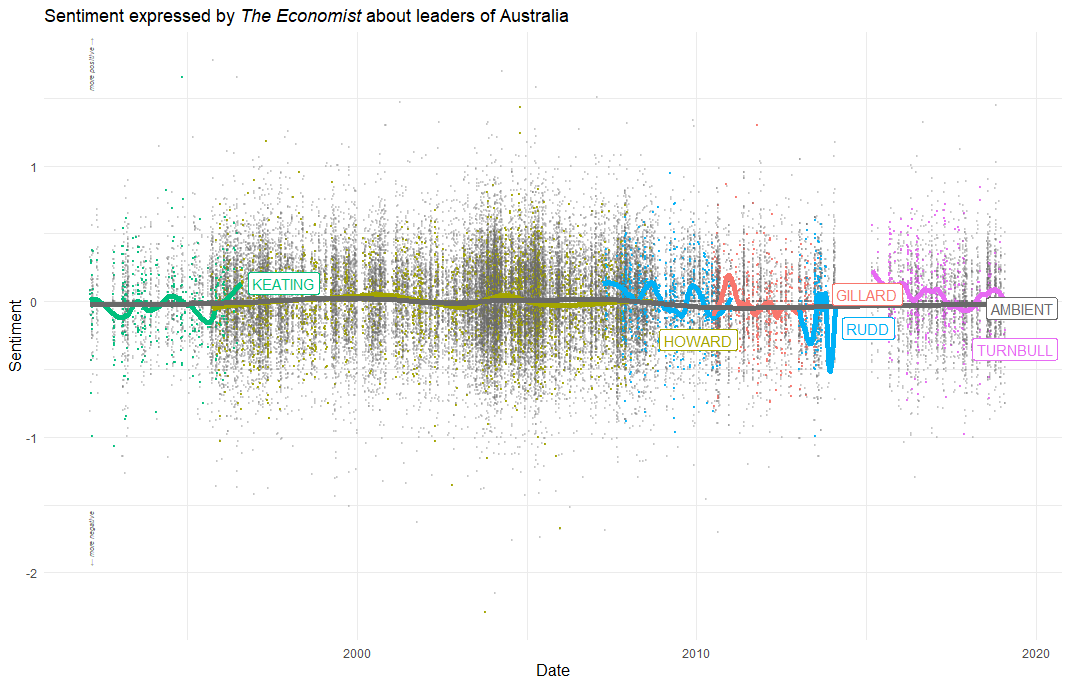
\includegraphics[width=\textwidth]{figures/900_timeline_fig.png}     
        \end{figure}

        Figure 1 illustrates two challenges. First, note that on average, SentimentR evaluates \textit{The Economist} as have almost perfectly neutral sentiment about most all leaders over time. The absence of heterogeneity is concerning for two reasons --- first that it is unlikely the case that \textit{The Economist} is truly neutral about these leaders given that it has a well-publicized \textit{ex ante} ideological position, and second that the absence of heterogeneity will make any regression analysis particularly sensitive to outliers.\footnote{Reading \textit{The Economist} is evidence enough that these very neutral scores are unrealistic and/or inaccurate.}

    \subsection{VADER}
        In light of the poor SentimentR results we turned to VADER to see if the valence-aware dictionary-based approach was worthwhile. In effect, I was testing to see if VADER and SentimentR produced different scores for the same sentences.\\

        Below, Figure 2 plots the correlation between VADER and SentimentR scores for selected Australian leaders. One of the features of VADER over SentimentR is that it preserves extreme values more often than does SentimentR. However, this property is symmetric at the sentence-level and entity-level observations are similarly clustered around 0 (perfectly neutral.)\\

        \begin{figure}[t]
            % \caption{SentimentR score vs. VADER score for selected Australian prime ministers}
            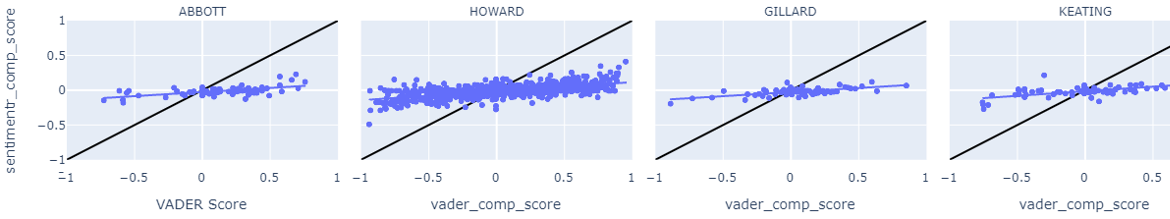
\includegraphics[width=\textwidth]{figures/AUS_VADER_SentimentR_Corels.png}
        \end{figure}

        A closer inspection of SentimentR and VADER results suggests that these tools are inadequate for the task at hand. Consider, for example, the following sentence from the July 7th, 2020, edition of the economist:
        \begin{quote}
            \singlespacing
            Brazil's president Jair Bolsonaro, who has downplayed the threat of COVID-19, flouted social-distancing guidelines and said that his ``athletic history'' would protect him, tested positive for the coronavirus.
        \end{quote} 
        
        SentimentR scores this sentence positively (0.426), largely due to the presence of of the word ``positive,'' when this sentence --- to a human reader --- clearly does not express a positive sentiment.\footnote{Even without context for what COVID-19 is, a human reader can identify the word ``flout'' as having a negative connotation. Additionally, in the medical context, testing ``positive'' for any kind of disease carries a negative connotation.} SentimentR and VADER lack knowledge of domain-specific idioms that can heavily weight the sentiment expressed in a sentence to the extremes. Because \textit{The Economist} writes about a wide variety of domains with the expectation that the reader is ``an educated layman,'' SentimetnR and VADER are inappropriate.

    \subsection{BART}
        Consequently we turned to BART, which is considerably more computationally intensive than are SentimentR and VADER, in the hope that more advanced techniques would produce results similar to an expert human reader.\\

        As noted above, at the article-, paragraph-, and sentence-level, BART returns a three-tuple of scores on the unit interval indicating the probability that the text segment of interest is closest to either ``Positive,'' ``Neutral,'' or ``Negative.'' To test whether BART was returning accurate sentiment evaluations, I assigned members of the research group 20 articles to score by hand so that results could be compared. Readers were asked to mark each article as being ``Very negative'' ``Negative,'' ``Neutral,'' ``Positive,'' or ``Very Positive.''\footnote{In some instances sentence- and paragraph-level text segments were also scored in the same fashion.} For purposes of comparison, I coerced BART scores into similar categories.\\

        Below, Table 1 contains pairwise Cohen's Kappa statistics that measure the degree of agreement between readers and/or BART. Additionally, because of the difficulty of interpreting the Kappa statistic, Table 2 outlines generally agreed-upon thresholds for what each statistic means.

        \begin{table}[ht]
            \centering
            \caption{Cohen's Kappa Statistic ($\kappa$) -- Inter-rater agreement}
            \resizebox*{\textwidth}{!}{
            \begin{tabular}{rcccccccccc}
            \hline
            \multicolumn{1}{l}{} &
              \textbf{BART\_FIVE} &
              \textbf{LUIGI} &
              \textbf{TANO} &
              \textbf{FABIO} &
              \textbf{FEDRICO} &
              \textbf{RACHEL} &
              \textbf{UTSAV} &
              \textbf{KHWAJA} &
              \textbf{JOSHUA} &
              \multicolumn{1}{l}{\textbf{RP AVG. (FIVE)}} \\ \hline
            \textbf{BART\_FIVE}                         & 1.0000 &        &        &        & 0.1028 & 0.2105 & 0.1638 & 0.1419 & 0.0841 & 0.0315 \\
            \textbf{LUIGI}                              &        & 1.0000 &        &        &        &        &        &        &        &        \\
            \textbf{TANO}                               &        &        & 1.0000 &        &        &        &        &        &        &        \\
            \textbf{FABIO}                              &        &        &        & 1.0000 &        &        &        &        &        &        \\
            \textbf{FEDERICO}                           &        &        &        &        & 1.0000 & 0.5238 & 0.1696 & 0.3506 & 0.2809 & 0.6601 \\
            \textbf{RACHEL}                             &        &        &        &        &        & 1.0000 & 0.2105 & 1.0000 & 1.0000 & 0.7368 \\
            \textbf{UTSAV}                              &        &        &        &        &        &        & 1.0000 & 0.3728 & 0.2715 & 0.4946 \\
            \textbf{KHWAJA}                             &        &        &        &        &        &        &        & 1.0000 & 0.6689 & 0.6564 \\
            \textbf{JOSHUA}                             &        &        &        &        &        &        &        &        & 1.0000 & 0.5235 \\
            \multicolumn{1}{l}{\textbf{RP AVG. (FIVE)}} &        &        &        &        &        &        &        &        &        & 1.0000 \\ \hline
            \end{tabular}
            }
        \end{table}

        \begin{table}[ht]
                \centering
                \caption{Cohen's Kappa Statistic ($\kappa$) -- Inter-rater agreement Coefficient Interpretation}
                % \resizebox*{\textwidth}{!}{
                    \begin{tabular}{@{}cc@{}}
                        \toprule
                        \multicolumn{1}{c}{\textbf{Kappa value ($\kappa$)}} & \multicolumn{1}{c}{\textbf{Interpretation}} \\ \midrule
                        \textless{}0 & Less than chance agreement \\
                        0-0.2        & Slight agreement           \\
                        0.2-0.4      & Fair agreement             \\
                        0.4-0.6      & Moderate agreement         \\
                        0.6-0.8      & Substantial agreement      \\
                        0.8-1        & Almost perfect agreement   \\ \bottomrule
                        \end{tabular}
                % }
        \end{table}

        These results are discussed at greater length below.

\section{Challenges}
    As evidenced by the inter-rater agreement statistics presented in Table 1, evaluating the sentiment of article published by \textit{The Economist} is difficult, even for human readers. That is, because the sentiment expressed by \textit{The Economist} is indicated by subtle cues, it is hard for humans to regularly and consistently agree upon the sentiment expressed about a leader.\\

    In particular, the purpose of this project is to identify something that is very abstract and very diffuse: the sentiment of \textit{The Economist's} evaluation of a leader and/or his or her policies. These layers of abstraction require an extraordinary amount of context about the issue domain that is the subject matter of a given article, \textit{The Economist's} regular editorial position, any deviation that the \textit{The Economist} might take from its regular position, domain-specific idioms, and a familiarity with the authorial voice and style used by \textit{The Economist}.\\

    Individually, these problems might be tractable. Taken together however, they pose a challenge that I have identified in four parts. The remainder of this section will focus on interpreting BART results (even if the challenges identified also apply to the SentimentR/VADER approach).\footnote{For ease of reading, this section might best be read with \texttt{BART\_SCORING\_SMOOTH\_COLORS.html} and/or the Google sheet open.}
    
    \subsection{Higher-resolution segment (un)certainty}
        A \textit{prima facie} inspection suggests BART results might be encouraging. At the article-level, the highest scores (used to identify the ``categorical'' score for a text segment) tend to reflect the general tone of the article. Additionally, these scores are often returned with a considerable degree of certainty. That is, BART evaluates an article as being considerably more likely to belong to a single cluster than to the other two.\footnote{A notable exception to this is the article about Spanish Prime Minister Jose Luis Rodriguz Zapatero, about which BART thinks the article is either quite positive or quite negative be definitely not neutral.}\\

        However, when evaluating text segments at the paragraph- or sentence-level, BART scores moderate across the three categories (i.e. BART is much less sure of which cluster a paragraph or sentence might belong to) or tend to the extremes without obvious (to humans) reason. With respect to the first problem, consider a sentence in an article about Emmanuel Macron published on September 30, 2017:
        
        \begin{quote}
            Having had no seats, Alternative for Germany, a disruptive and polarising force, is now the Bundestag's third largest party.
        \end{quote}

        Because BART lacks domain specific context and knowledge about \textit{The Economist's}position on the AfD, BART is very uncertain about which category this sentence belongs to. By contrast, a human reader would likely mark this sentence as ``negative'' or ``very negative.''\\

        On the other hand, in an article published in 2002 about European political shifts, the sentence ``What is true of Germany is true of the rest of Europe,'' is scored very confidently positively even though it is unclear to a human reader why this is the case. This problem, when taken together with leader reference ambiguity problem (described below), poses a considerable challenge.

    \subsection{Disaster/event and Affect bias}
        Though it does appear to identify semantically relevant evaluations of sentiment more distinctly and accurately than does SentimentR or VADER, BART still suffers from a disaster/affect bias in its evaluation of articles. Take for instance an article about a nuclear disaster in Japan and prime minister Obuchi Keizo's response. BART identifies the article as being broadly negative --- in large part, it appears, because of the mention of nuclear disaster. BART is unable, however, to readily distinguish the relatively neutral sentiment about Obuchi's response to the nuclear disaster, from the apocalyptic language used to describe the disaster itself. This is a problem that cannot obviously be resolved without conducting sentiment analysis with higher-resolution text segments, which itself (as described above) is beset by problems.

    \subsection{Leader reference ambiguity}
        Most articles published by \textit{The Economist} do not cleanly identify a single leader That is, articles are not profiles. Instead, articles often draw comparisons against other world leaders, domestic political allies and adversaries, business leaders, and other notable figures. Thus, it is inappropriate to take the sentiment score (or categorization) of an article and suppose that score is actually reflective of \textit{The Economist's} opinion of a leader of interest.\\

        Consider the September 2017 article published about Angela Merkel. This article is largely laudatory of her and hopeful for her fourth term as chancellor of Germany. (BART and most human readers agree that this article is generally positive.) However, this article also mentions Donald Trump and Vladimir Putin  --- and, by our current procedure --- this would be identified as a Trump article and a Putin article in addition to a Merkel article. The first three sentences of the article, open as follows:

        \begin{quote}
            To her many fans, Angela Merkel is the hero who stands up to Donald Trump and Vladimir Putin,, and who generously opened her country to refugees. To others she is the villain whose ill-thought-out gamble on immigration is ``ruining Germany,'' as Mr Trump once put it, and whose austerity policies laid waste to southern Europe. The fans are closer to the truth.\footnote{BART currently scores the first sentence very positively, the second sentence very negatively, and the third sentence mixed between positive and neutral. Though this seems like correct scoring with Merkel as the primary entity, note that the reverse is true for Trump and Putin.}
        \end{quote}

        This leader ambiguity problem is consistent across many types of articles, particularly those that focus on bilateral relations. A potential solution would be to tag an article as being associated with a leader only if the the leader cluster appears in a number of spans greater than some pre-determined threshold. To my mind this would be inappropriate for two reasons. First, this is likely to remove large parts of the sample for leaders who are only mentioned a small number of times by \textit{The Economist} or remove leaders from the sample entirely. Second, the style of \textit{The Economist} is often to moderate the language of its evaluation of a leader when an article is primarily about a leader by offering nuance, but be more explicit when a leader is not the primary subject.\footnote{This problem is given further treatment in section 6.} In the case of the Merkel article, a human reader can identify that the first three sentences are laden with seniment-weighted language. That is, even if --- as in the case of Trump and Putin --- there are many articles in the corpus that mention a leader, observations like the one above are valuable and should be preserved in the corpus because they tip \textit{The Economist's} hand.\footnote{Taken in conjunction with the high-resolution uncertainty problem descibed above however, this becomes doubly hard. Ideally, these highly sentiment-salient sentences could be identified and extracted as being the most important parts of an article. But, BART performs poorly on high-resolution text segments.}\\

    \subsection{Leader-policy-colleague metynomic ambiguity}
        Humans and BART alike struggle with the problem of how to assess \textit{The Economist's} evaluation of leader with respect to the attribution of successes/failures to a leader of interest, a leader's policies, a leader's (cabinet) colleagues, etc. That is, BART does poorly at evaluating sentences that are salient to a leader's ideological position but do only indirectly reference a leader.\\

        Take, for instance, a 2018 article about Spanish Prime Ministers Mariano Rajoy and Pedro Sanchez that in part reads as follows:

        \begin{quote}
            The new prime minister has not offered to repeal Mr Rajoy's liberalising labour market reform, as the unions would like. This reform has helped to spur a rapid fall in unemployment during the past four years of strong economic recovery from the euro crisis. All this means that the political shake-up has caused scarcely a ripple among investors, who are more concerned with Italy's political crisis.
        \end{quote}

        The construction of this paragraph makes reading comprehension and sentiment analysis (with respect to Rajoy and Sanchez) difficult. It is left to the reader to interpret \textit{The Economist's} position on labor market reforms and to what degree ``not [offering] to repeal'' them reflects well or poorly on Rajoy (who implemented them) or Sanchez (who has merely yet to suggest repealing them). Because BART does not have access to external sources of context this is harder still.\\

        The same or similar problems proliferate rapidly because \textit{The Economist} comments on matters of politics, domestic policy, and international relations. This causes the number of relative comparisons or attributions to increase without an obvious way to weight the relative importance of these domains. Consider the case of a wide-ranging article about Manhmohan Singh, prime minister of India. The article opines on past performance as finance minister, current political predicaments, and a comparison of development policy with China. How should each of these pronouncements be weighted? Should this Singh-article receive a very positive score because it is optimistic about the potential for his reforms? Or should that score be moderated because despite positively assessed reforms, inability to achieve them suggests failure of competence? While this case might be easy to decide, the number of ``long-tail'' attributions makes accurate, systematic evaluation hard.

\section{The Case to End this (version of the) Project}

        A sentiment analysis tool, for the purposes of this project should have at least the following two desirable properties: First, it should at least be able to identify the most extreme evaluations. In the subset of 20 articles scored by BART the article about Bolsonaro reads to human readers as the most negative. BART however, only rates it as moderately negative (less negative than other articles). To my mind this is a meaningful failure. Inability to identify the most extreme values suggests that the underlying tool is likely to be inaccurate when dealing with more nuanced cases. Second, it should be able to identify the most important text segment(s) when evaluating an article at large. That is, \textit{The Economist} often concentrates sentiment-laden sentences or paragraphs together, even if the majority of the article contains relatively neutral fact-based or fact-like sentences.\footnote{Even if all sentences were pre-processed for fact-opinion distinction, the problem remains that \textit{The Economist} often uses statements of fact to cast negative aspersions about the performance of a leader, for instance in the midst of a crisis.} It would be a desirable trait of a sentiment analysis tool to segregate the most important sentiment-laden sentences/text segments from the neutral statements before evaluating them. That is currently out of reach of BART.\footnote{Additionally, trying to identify these most sentiment-laden sentences by hand is as hard as merely reading and scoring every article by humans.}\\

        It is my opinion that what we are asking of existing NLP tools remains out of reach. If \textit{The Economist} exhibited just one of the problems described above, this problem might be tractable. However, taken together, I do not think that the existing technology could accurately assess what we are trying to isolate (the sentiment of \textit{The Economist's} evaluation of a leader (and his/her policies)). The above problems do not exist in isolation from each other but are tightly connected and enmeshed. I think that this is borne out by the amount of disagreement among human readers. What we are trying to do is still hard for human readers and NLP techniques are not yet sufficiently advanced to replicate even human performance.\\

        This poor performance has a double penalty for us. First, an ``incorrect'' sentiment evaluation does not merely get dropped for the sample. It remains in the sample but incorrectly coded.\footnote{Unfortunately checking that the sentiment has been correctly coded is analogous to an NP-hard problem. That is, it is as hard to check for correctness as it is to evaluate sentiment correctly.} Second, any incorrectly coded observations may drive (incorrect) results in future (regression) analysis.\\

        Even if it was the case that a simple, highly accurate sentiment evaluation tool became rapidly available, we have yet to seriously consider the data collection process for response variables. A cursory inspection suggests that post-office compensation details are hard to systematically identify and may be inaccurate (becuase post-office earnings are not subject to any kind of disclosure rules or transparency norms). Making this problem doubly hard is the many different kinds of compensation that a former world leader might receive. For instance, how would one weight a large advance on a book deal against speaking fees? Should immediately-post-office earnings be weighted more or less heavily than delayed post-office earnings? Again, if these questions could be quickly answered, and present unreliability of the predictive variables (presently only \text{The Economist} sentiment evaluations) be quickly resolved, there remains less-than-one probability of identifying robust results.\\

        For these reasons, I am of the opinion that the outlook for this project is dim. Without considerable advancement in methods, and with little guarantee of robust results, I think that the probability of success is low. 
    
\end{document}